\documentclass[12pt]{article}
\usepackage[margin=1in]{geometry}
\usepackage[utf8]{inputenc}
\usepackage[T1]{fontenc}
\usepackage{graphicx}
\usepackage{tabularx}
\usepackage{booktabs}
\usepackage{enumitem}
\usepackage{hyperref}
\usepackage{fancyhdr}
\usepackage{lastpage}
\usepackage{xcolor}
\usepackage{subcaption}
\usepackage{float}
\usepackage{cite}
\usepackage{amsmath,amssymb,amsfonts}
\usepackage{algorithmic}
\usepackage{textcomp}
\usepackage{multirow}
\usepackage{url}
\usepackage{setspace}
\usepackage{titlesec}

% Define university color (minimal use)
\definecolor{munimaroon}{RGB}{128,0,0}

% Format section titles with maroon color
\titleformat{\section}
  {\normalfont\Large\bfseries\color{munimaroon}}
  {\thesection}{1em}{}
\titleformat{\subsection}
  {\normalfont\large\bfseries\color{munimaroon}}
  {\thesubsection}{1em}{}

% Header and footer configuration
\pagestyle{fancy}
\fancyhf{}
\fancyhead[L]{\small MUNI University EHRMS Proposal}
\fancyhead[R]{\small \today}
\fancyfoot[C]{\small Page \thepage\ of \pageref{LastPage}}
\renewcommand{\headrulewidth}{0.5pt}
\renewcommand{\footrulewidth}{0.5pt}

% Hyperlink setup
\hypersetup{
    colorlinks=true,
    linkcolor=black,
    urlcolor=blue,
    citecolor=black,
    pdfborder={0 0 0}
}



\begin{document}

% Custom Title Page
\begin{titlepage}
    \centering
    \vspace*{1cm}
    
    
\includegraphics[width=4cm]{muni-logo.jpg}
    
    \vspace{1.5cm}
    
    {\Huge \textbf{\color{munimaroon}ELECTRONIC HUMAN RESOURCE}} \\
    \vspace{0.3cm}
    {\Huge \textbf{\color{munimaroon}MANAGEMENT SYSTEM}} \\
    \vspace{0.5cm}
    {\LARGE \textbf{(EHRMS)}} \\
    
    \vspace{1cm}
    {\color{munimaroon}\rule{0.8\textwidth}{1pt}}
    \vspace{0.5cm}
    
    {\Large \textbf{Development Proposal}} \\
    \vspace{0.3cm}
    {\large \color{munimaroon}Muni University}
    
    \vfill
    
    {\large \textbf{Prepared by:}} \\
    \vspace{0.3cm}
    {\large Muhindo Mubarak} \\
    \textit{Application Engineer \& Full Stack Developer} \\
    \vspace{0.3cm}
    \small muhindo@8technologies.net | +256 783 204 665
    
    \vspace{1cm}
    
    {\large November 30, 2025}
    
\end{titlepage}

% Table of Contents
\tableofcontents
\newpage

\section*{Executive Summary}

Muni University seeks to modernize its human resource management infrastructure through the implementation of a comprehensive Electronic Human Resource Management System (EHRMS). This proposal outlines the development of an integrated digital platform that will revolutionize HR operations through automation, enhanced security, and data-driven decision-making.

The proposed EHRMS will comprise five strategically designed core modules, seamlessly integrated with state-of-the-art touchless facial recognition technology. This advanced biometric solution will ensure secure, contactless authentication while providing real-time attendance tracking capabilities. The system is designed to eliminate manual processes, reduce administrative overhead, and provide actionable insights through comprehensive analytics and reporting features.

By implementing this solution, Muni University will achieve operational excellence in workforce management, improved compliance with statutory requirements, enhanced employee experience, and significant cost savings through process automation. The system will serve as a centralized hub for all HR-related activities, fostering transparency, accountability, and efficiency across the institution.

\section{Background and Justification}

\subsection{Current Challenges}

Muni University currently faces several challenges in human resource management that necessitate the adoption of a modern, integrated EHRMS:

\begin{itemize}[noitemsep]
\item \textbf{Manual Record-Keeping:} Paper-based personnel files result in inefficiencies, difficulty in information retrieval, and increased risk of data loss.
\item \textbf{Time-Consuming Processes:} Manual attendance tracking and leave management consume significant administrative time and resources.
\item \textbf{Limited Analytics:} Absence of real-time HR metrics and analytics hampers strategic workforce planning and decision-making.
\item \textbf{Security Concerns:} Traditional attendance systems are vulnerable to proxy attendance and time fraud.
\item \textbf{Compliance Issues:} Manual processes make it challenging to maintain accurate records for statutory compliance and auditing purposes.
\item \textbf{Employee Dissatisfaction:} Cumbersome leave application processes and lack of self-service options affect employee satisfaction.
\end{itemize}

\subsection{Strategic Objectives}

The implementation of the EHRMS aligns with the university's strategic goals to:

\begin{itemize}[noitemsep]
\item Enhance operational efficiency through digital transformation of HR processes
\item Improve data accuracy, security, and accessibility across the institution
\item Enable evidence-based decision-making through comprehensive workforce analytics
\item Foster a culture of transparency and accountability in human resource management
\item Position the university as a leader in adopting modern management technologies
\item Reduce operational costs associated with manual HR administration
\end{itemize}

\section{Project Overview}

\subsection{System Description}

The Muni University EHRMS is a comprehensive, cloud-ready platform designed to serve as the central repository for all human resource information and operations. The system employs a modular architecture that ensures scalability, maintainability, and ease of integration with existing university systems.

Built on modern web technologies and industry best practices, the EHRMS will provide role-based access to administrators, department heads, HR personnel, and employees. The platform features an intuitive user interface, responsive design for mobile accessibility, and robust security measures to protect sensitive personnel information.

\subsection{Key Benefits}

\begin{enumerate}[noitemsep]
\item \textbf{Operational Efficiency:} Automation of routine HR tasks reduces administrative workload by an estimated 60-70\%.
\item \textbf{Enhanced Security:} Biometric authentication eliminates buddy punching and ensures accurate attendance records.
\item \textbf{Cost Savings:} Reduction in paper usage, storage costs, and administrative overhead translates to significant long-term savings.
\item \textbf{Improved Compliance:} Automated record-keeping ensures adherence to statutory requirements and simplifies audit processes.
\item \textbf{Employee Empowerment:} Self-service portals enable employees to manage their information, apply for leave, and track attendance independently.
\item \textbf{Data-Driven Decisions:} Real-time analytics and reporting provide insights for strategic workforce planning and resource allocation.
\item \textbf{Scalability:} The modular architecture allows for future expansion and integration of additional HR functions as needed.
\end{enumerate}

\section{Core System Modules}

\subsection{Module 1: Employee Basic Information Management}

This foundational module serves as the central repository for all employee-related information, providing a comprehensive digital personnel management system.

\textbf{Key Features:}
\begin{itemize}[noitemsep]
\item Centralized employee database with detailed profiles including biographical data, photographs, and unique identifiers
\item Digital document management system for storing contracts, certificates, transcripts, and other personnel documents
\item Complete employment history tracking including positions held, promotions, transfers, and salary progressions
\item Academic and professional qualifications registry with automated expiry notifications for certifications
\item Emergency contact information and next-of-kin details management
\item Dependent information tracking for benefits administration purposes
\item Bank account details and payroll information management
\item Department and organizational unit assignment with hierarchical structure
\item Employee search and filtering capabilities with advanced query options
\item Bulk import and export functionality for data migration and reporting
\end{itemize}

\textbf{Access Control:}
\begin{itemize}[noitemsep]
\item HR administrators: Full read/write access
\item Department heads: View access for their department staff
\item Employees: View and limited update access to own information
\end{itemize}

\subsection{Module 2: Clocking and Attendance Management}

This module leverages cutting-edge facial recognition technology to provide a touchless, secure, and accurate time and attendance tracking system.

\textbf{Key Features:}
\begin{itemize}[noitemsep]
\item Touchless facial recognition for contact-free clock-in and clock-out
\item Real-time attendance monitoring with live dashboard displays
\item Automated timesheet generation with accurate work hours calculation
\item Late arrival and early departure detection with configurable thresholds
\item Overtime tracking and calculation based on institutional policies
\item Shift management and scheduling capabilities
\item Multiple location support for distributed campus operations
\item Mobile application for field staff attendance marking with GPS verification
\item Exception management for handling missed clocks and attendance corrections
\item Integration with payroll systems for accurate compensation processing
\item Comprehensive attendance reports with customizable date ranges and filters
\item Automated email notifications for attendance violations and anomalies
\end{itemize}

\textbf{Device Integration:}

The system will integrate seamlessly with DS-K1T680DF-E1 facial recognition terminals deployed at strategic locations across the campus. These devices will communicate with the central EHRMS through secure RESTful APIs, ensuring real-time data synchronization.

\subsection{Module 3: Leave Management}

A comprehensive leave administration system designed to automate the entire leave lifecycle from application to approval and balance tracking.

\textbf{Key Features:}
\begin{itemize}[noitemsep]
\item Intuitive leave application interface with calendar view
\item Configurable approval workflows with multi-level authorization
\item Automatic leave balance calculation and accrual tracking
\item Support for multiple leave types including:
  \begin{itemize}
  \item Annual/Vacation Leave
  \item Sick Leave
  \item Maternity/Paternity Leave
  \item Study Leave
  \item Compassionate Leave
  \item Leave Without Pay
  \item Public Holidays
  \end{itemize}
\item Leave policy engine for defining institution-specific rules and entitlements
\item Leave calendar with team visibility for effective resource planning
\item Manager approval portal with delegation capabilities
\item Email notifications for leave requests, approvals, and rejections
\item Leave reports including utilization, pending requests, and forecasting
\item Mobile app integration for on-the-go leave applications
\item Carry-forward and leave encashment calculations
\item Integration with attendance system for automatic leave marking
\end{itemize}

\subsection{Module 4: Review and Appraisal Management}

A structured performance management system designed to facilitate continuous employee development and objective performance evaluation.

\textbf{Key Features:}
\begin{itemize}[noitemsep]
\item Customizable performance evaluation templates aligned with university objectives
\item SMART goal setting framework (Specific, Measurable, Achievable, Relevant, Time-bound)
\item Configurable appraisal cycles (quarterly, bi-annual, annual)
\item 360-degree feedback mechanism incorporating input from supervisors, peers, and subordinates
\item Competency assessment framework with rating scales
\item Performance improvement plan (PIP) tracking for underperforming employees
\item Self-assessment capabilities for employee participation
\item Performance analytics and trend analysis over multiple appraisal periods
\item Career development planning and succession management tools
\item Training needs identification based on performance gaps
\item Performance-based reports for promotion and compensation decisions
\item Document attachment support for evidence-based evaluations
\item Automated reminders for pending appraisals and review deadlines
\end{itemize}

\subsection{Module 5: Reporting and Analytics}

A powerful business intelligence module providing comprehensive insights into workforce metrics and HR operations.

\textbf{Key Features:}
\begin{itemize}[noitemsep]
\item Executive HR dashboard with key performance indicators (KPIs):
  \begin{itemize}
  \item Headcount and workforce composition
  \item Attendance rates and patterns
  \item Leave utilization statistics
  \item Performance distribution
  \item Turnover and retention metrics
  \end{itemize}
\item Interactive data visualization using charts, graphs, and heat maps
\item Customizable report builder with drag-and-drop functionality
\item Scheduled report generation and automated email distribution
\item Workforce analytics including demographic analysis, age distribution, and tenure statistics
\item Attendance analytics with trends, patterns, and anomaly detection
\item Leave analytics including forecasting and capacity planning
\item Performance metrics and correlation analysis
\item Compliance reporting for statutory requirements
\item Export functionality to PDF, Excel, and CSV formats
\item Data filtering, sorting, and drill-down capabilities
\item Real-time data refresh for up-to-date information
\item Role-based report access ensuring data confidentiality
\end{itemize}

\section{Hardware Requirements}

\subsection{Facial Recognition Terminals}

The system will utilize high-performance, touchless facial recognition devices specifically designed for accurate biometric authentication in diverse environmental conditions.

\begin{figure}[H]
\centering
\begin{subfigure}{0.3\textwidth}
    \centering
    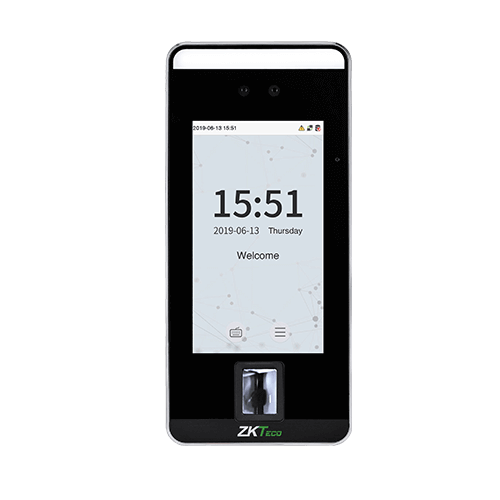
\includegraphics[width=\linewidth]{face-rec-1.png}
    \caption{Front View}
\end{subfigure}
\hfill
\begin{subfigure}{0.3\textwidth}
    \centering
    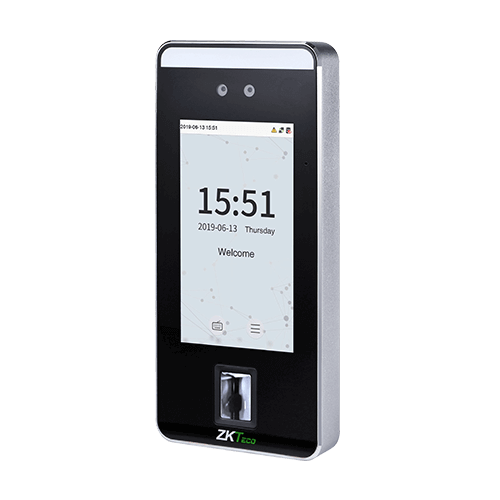
\includegraphics[width=\linewidth]{face-rec-2.png}
    \caption{Display Interface}
\end{subfigure}
\hfill
\begin{subfigure}{0.3\textwidth}
    \centering
    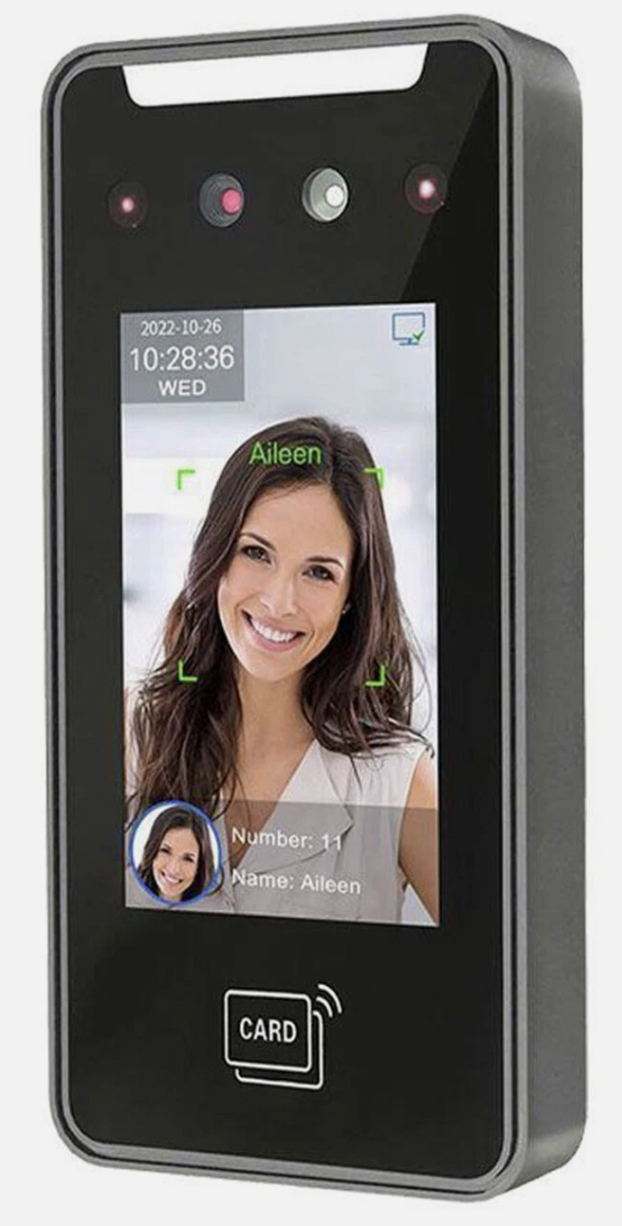
\includegraphics[width=\linewidth]{face-rec-3.png}
    \caption{Installation View}
\end{subfigure}
\caption{DS-K1T680DF-E1 Facial Recognition Terminals}
\end{figure}

\begin{table}[H]
\centering
\begin{tabularx}{\textwidth}{lX}
\toprule
\textbf{Specification} & \textbf{Details} \\
\midrule
Model & DS-K1T680DF-E1 Advanced Facial Recognition Terminal \\
Display & 8-inch high-resolution capacitive touch screen LCD \\
User Interface & Intuitive capacitive touch screen operation \\
Camera System & Dual lens configuration with 2 MP resolution \\
 & Wide dynamic range (WDR) for varying light conditions \\
Field of View & Horizontal: 88° | Vertical: 44° | Diagonal: 108° \\
Recognition Distance & 0.3m to 1.5m (optimized for doorway installations) \\
Recognition Speed & $<$ 0.2 seconds per identification \\
Face Capacity & Up to 50,000 face templates \\
Recognition Accuracy & $>$ 99\% in optimal conditions \\
Network Connectivity & 10/100/1000M Ethernet (RJ-45) \\
 & TCP/IP, HTTP, HTTPS protocols \\
Integration Interfaces & Lock control relay output \\
 & Exit button input \\
 & Door contact sensor input \\
 & Alarm inputs (2 channels) \\
 & Alarm output (1 channel) \\
 & Tamper detection \\
 & RS-485 (Wiegand protocol support) \\
 & USB interface for firmware updates \\
Card Authentication & DESFire card support \\
 & Felica card compatibility \\
 & Multi-factor authentication capability \\
Power Requirements & 12-24 VDC, 3A (standard) \\
 & IEEE 802.3af PoE support (optional) \\
Operating Temperature & -30°C to 60°C (industrial grade) \\
Operating Humidity & 0\% to 90\% (non-condensing) \\
Protection Rating & IP65 (dust-tight and water-resistant) \\
Dimensions & 145mm (W) × 145mm (H) × 35mm (D) \\
Installation & Wall-mounted with included bracket \\
Certifications & CE, FCC compliant \\
\bottomrule
\end{tabularx}
\caption{Facial Recognition Terminal Specifications}
\end{table}

\subsection{Recommended Deployment}

For comprehensive coverage of Muni University's operations, we recommend the following terminal deployment strategy:

\begin{itemize}[noitemsep]
\item \textbf{Main Administration Building:} 2 terminals (entry and exit points)
\item \textbf{Faculty Buildings:} 1 terminal per major faculty building (estimated 4-6 units)
\item \textbf{Library:} 1 terminal at main entrance
\item \textbf{Staff Common Areas:} 1 terminal for central monitoring
\item \textbf{Security Gates:} 2 terminals at main university entrances
\end{itemize}

\textit{Note: The exact number and placement of terminals will be determined during the site assessment phase to optimize coverage and cost-effectiveness.}

\section{System Interface Screenshots}

\subsection{Login Portal}

The EHRMS features a professional, university-branded login interface with secure authentication.

\begin{figure}[H]
\centering
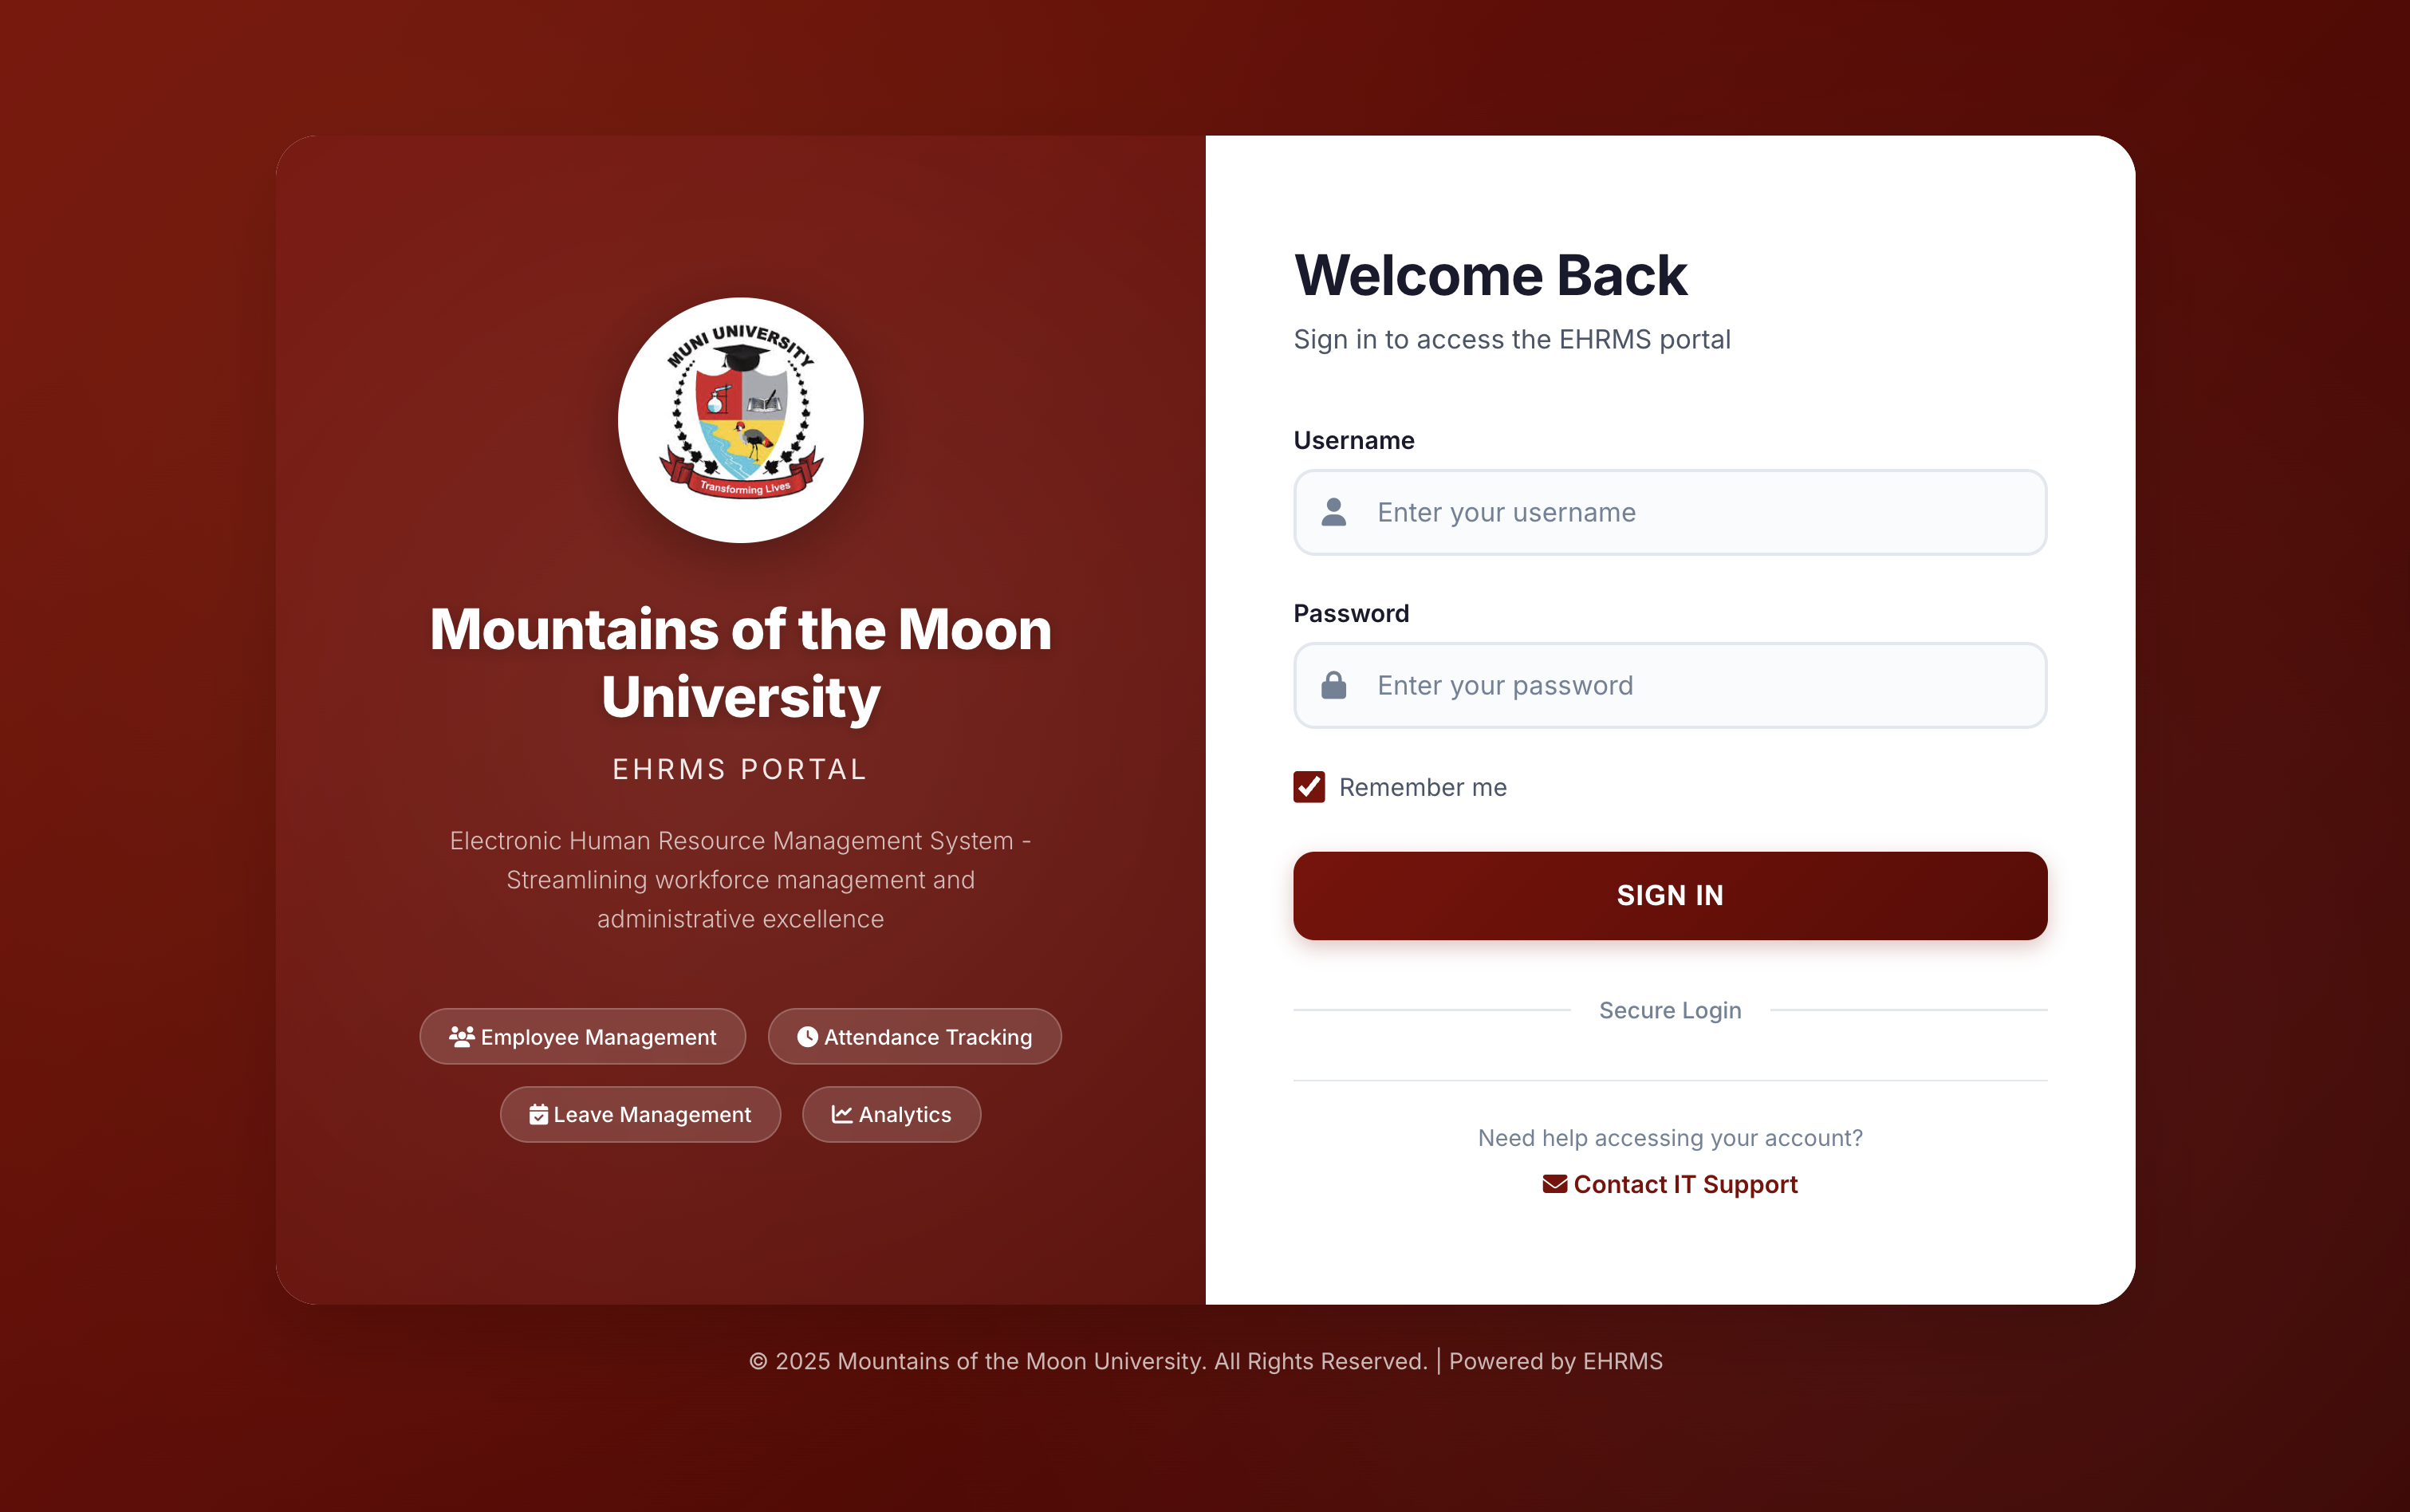
\includegraphics[width=\textwidth]{muni-login-1.png}
\caption{EHRMS Login Portal - Muni University Branded Interface}
\end{figure}

\subsection{Dashboard Interface}

The system provides an intuitive, data-rich dashboard with comprehensive HR analytics and key performance indicators.

\begin{figure}[H]
\centering
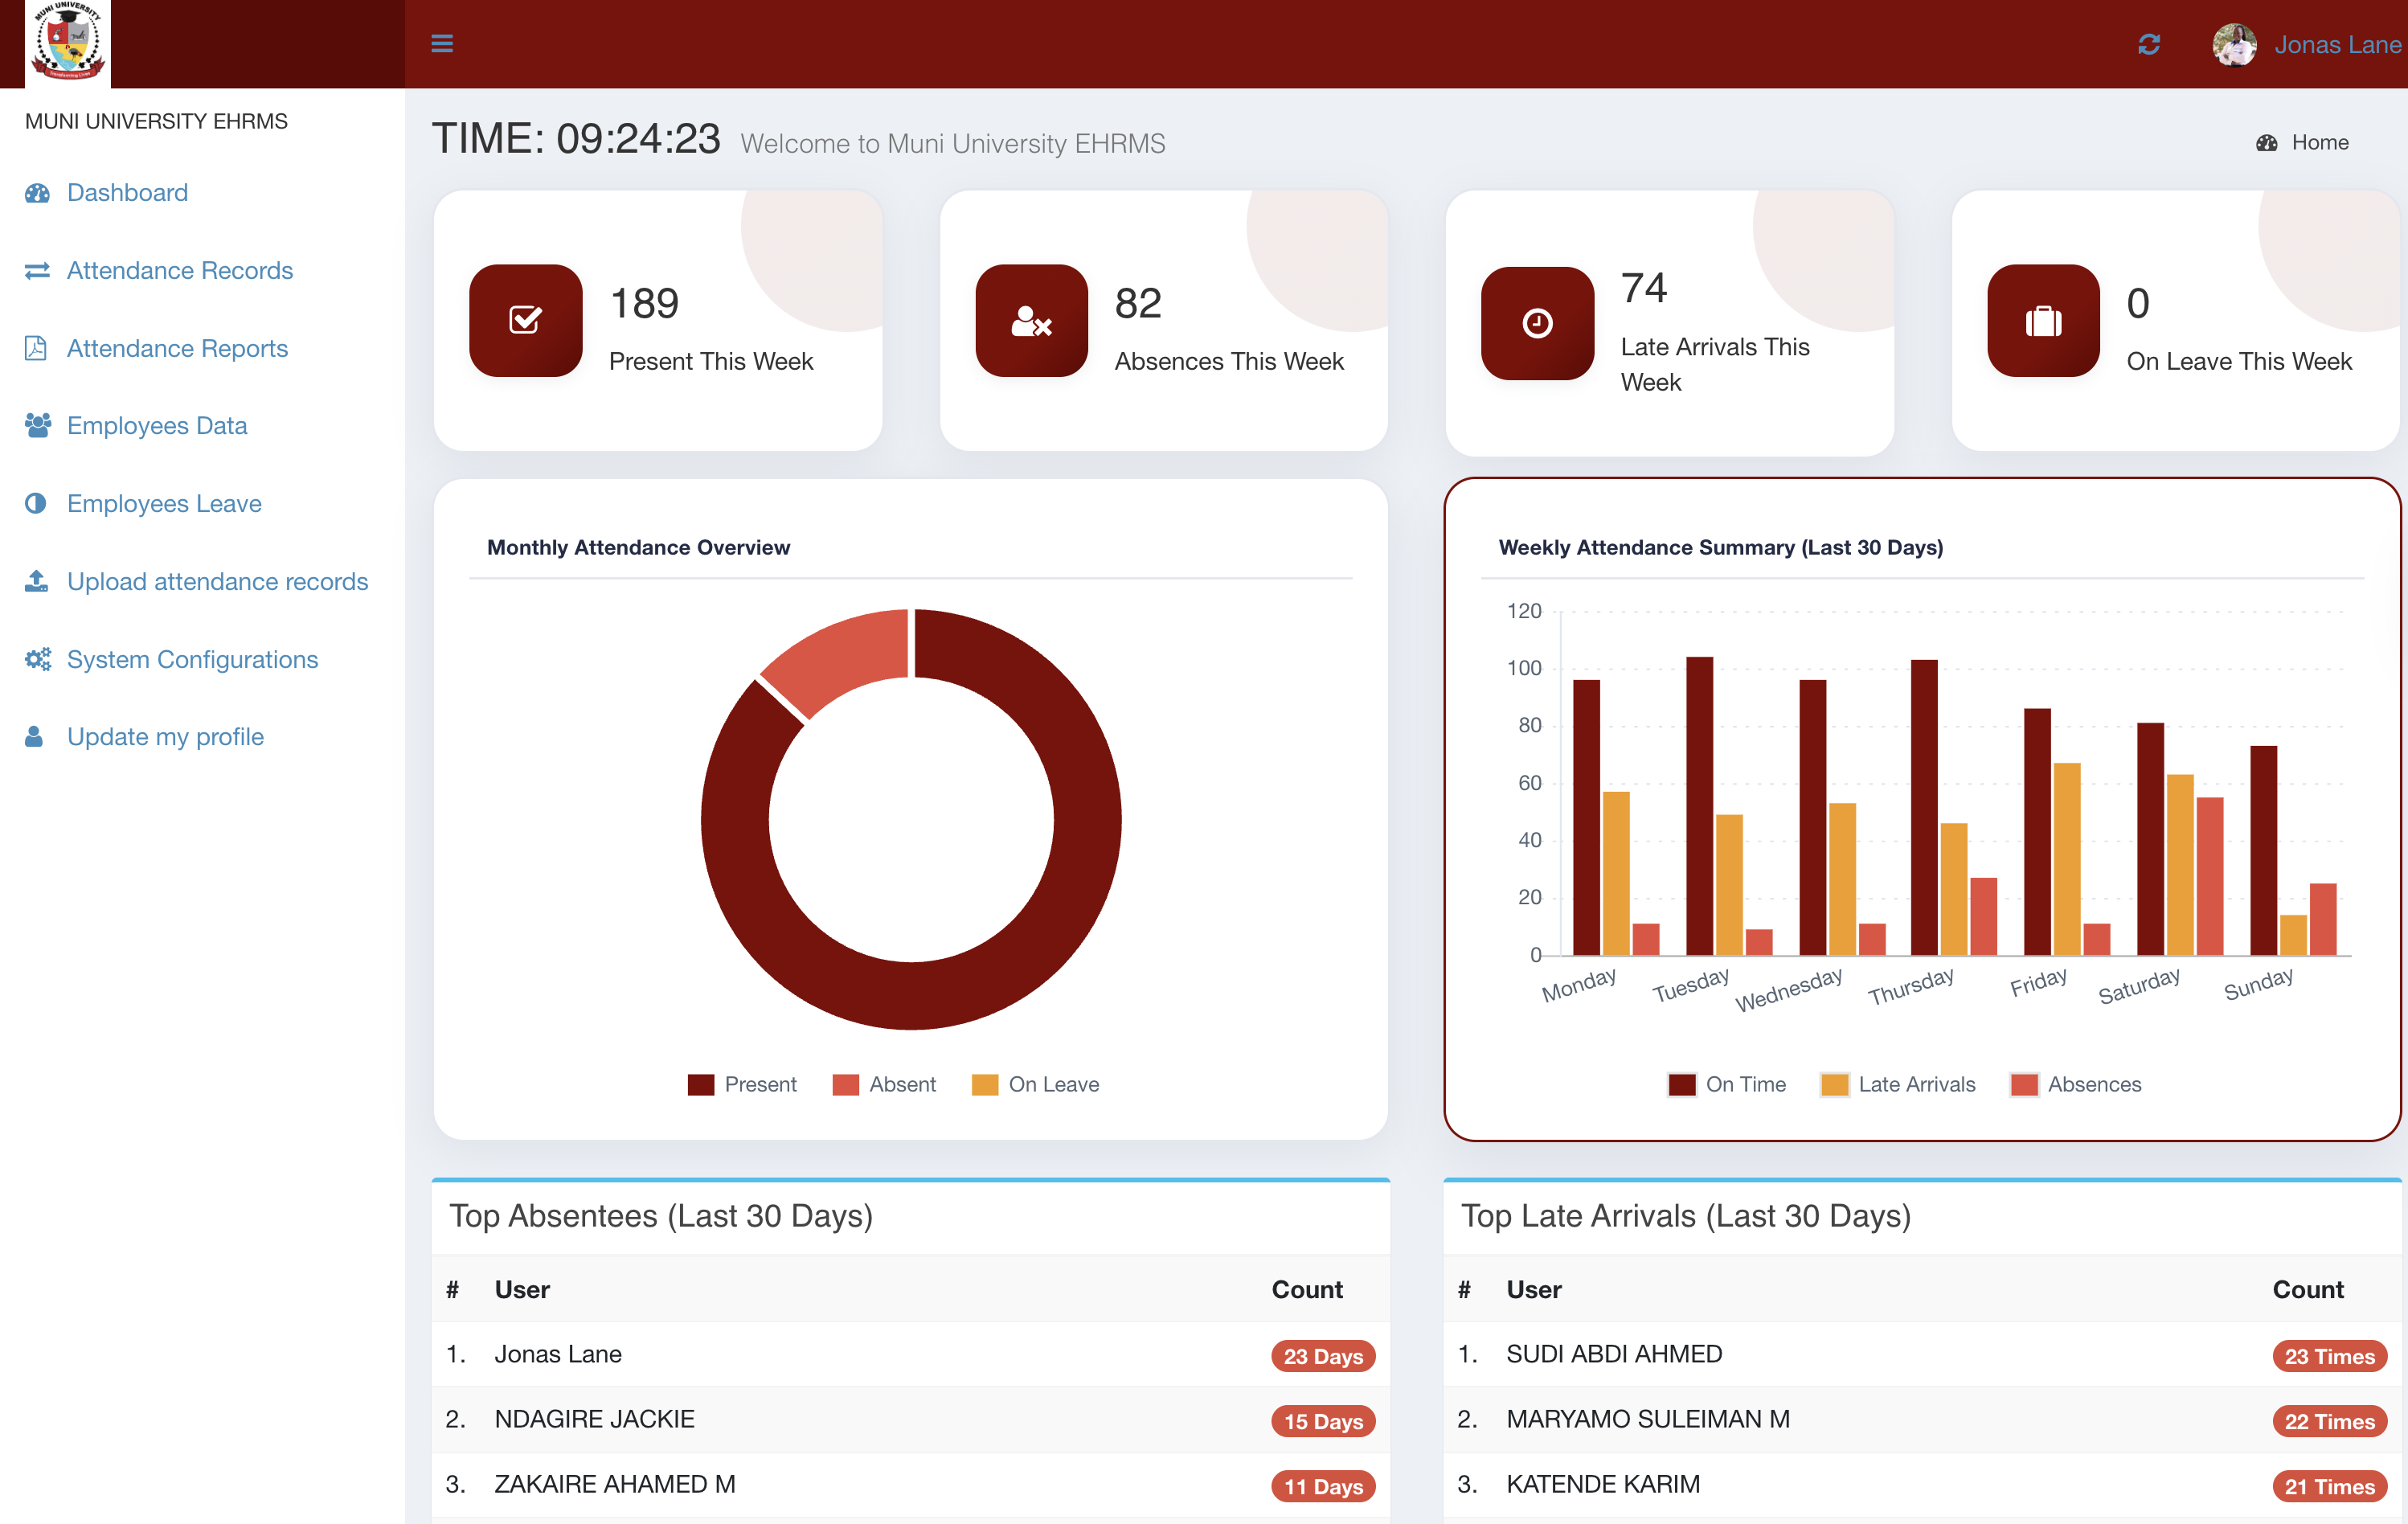
\includegraphics[width=\textwidth]{muni-dashboard-2.png}
\caption{EHRMS Dashboard - Real-time HR Analytics and Metrics}
\end{figure}

\section{Technical Architecture and Implementation}

\subsection{Technology Stack}

The EHRMS will be built using modern, industry-standard technologies ensuring reliability, performance, and long-term maintainability.

\textbf{Frontend Technologies:}
\begin{itemize}[noitemsep]
\item \textbf{Web Application:} React.js 18+ with TypeScript for type safety
\item \textbf{UI Framework:} Material-UI (MUI) for consistent, professional interface design
\item \textbf{State Management:} Redux Toolkit for efficient application state handling
\item \textbf{Data Visualization:} Chart.js and D3.js for interactive analytics
\item \textbf{Responsive Design:} Mobile-first approach ensuring accessibility across all devices
\end{itemize}

\textbf{Backend Technologies:}
\begin{itemize}[noitemsep]
\item \textbf{Framework:} Python Django 4.2+ with Django REST Framework
\item \textbf{API Architecture:} RESTful API design with comprehensive documentation
\item \textbf{Authentication:} JWT (JSON Web Tokens) for secure session management
\item \textbf{Task Queue:} Celery with Redis for asynchronous processing
\item \textbf{Real-time Communication:} Django Channels for WebSocket support
\end{itemize}

\textbf{Database and Storage:}
\begin{itemize}[noitemsep]
\item \textbf{Primary Database:} PostgreSQL 15+ for relational data integrity
\item \textbf{Caching Layer:} Redis for improved performance
\item \textbf{File Storage:} AWS S3-compatible storage for documents and images
\item \textbf{Backup Strategy:} Automated daily backups with 30-day retention
\end{itemize}

\textbf{Mobile Application:}
\begin{itemize}[noitemsep]
\item \textbf{Framework:} Flutter 3.x for cross-platform development
\item \textbf{Platforms:} iOS and Android native compilation
\item \textbf{Features:} Push notifications, offline capability, biometric authentication
\end{itemize}

\textbf{Security Implementation:}
\begin{itemize}[noitemsep]
\item Role-Based Access Control (RBAC) with granular permissions
\item AES-256 encryption for sensitive data at rest
\item TLS 1.3 for data in transit
\item SQL injection and XSS attack prevention
\item CSRF token protection
\item Regular security audits and penetration testing
\item Comprehensive audit logging of all system activities
\end{itemize}

\textbf{DevOps and Deployment:}
\begin{itemize}[noitemsep]
\item \textbf{Version Control:} Git with branching strategy
\item \textbf{CI/CD Pipeline:} Automated testing and deployment
\item \textbf{Containerization:} Docker for consistent deployment environments
\item \textbf{Orchestration:} Docker Compose or Kubernetes for production
\item \textbf{Monitoring:} Application performance monitoring and error tracking
\item \textbf{Logging:} Centralized logging with ELK stack (Elasticsearch, Logstash, Kibana)
\end{itemize}

\subsection{System Architecture}

The EHRMS follows a three-tier architecture pattern:

\begin{enumerate}[noitemsep]
\item \textbf{Presentation Layer:} React.js web application and Flutter mobile apps
\item \textbf{Application Layer:} Django REST API with business logic implementation
\item \textbf{Data Layer:} PostgreSQL database with optimized schema design
\end{enumerate}

This architecture ensures separation of concerns, facilitates independent scaling of components, and simplifies maintenance and future enhancements.

\section{Project Deliverables}

Upon successful completion of the project, the following deliverables will be provided to Muni University:

\subsection{Software Deliverables}

\begin{enumerate}
\item \textbf{Web Application:}
   \begin{itemize}[noitemsep]
   \item Fully functional EHRMS web portal accessible via modern browsers
   \item Responsive design supporting desktop, tablet, and mobile access
   \item Role-based dashboards for administrators, managers, and employees
   \end{itemize}

\item \textbf{Mobile Applications:}
   \begin{itemize}[noitemsep]
   \item Native Android application (APK and Google Play Store deployment)
   \item Native iOS application (IPA and Apple App Store deployment)
   \item Employee self-service features including leave applications and attendance viewing
   \item Push notification support for alerts and approvals
   \end{itemize}

\item \textbf{Device Integration:}
   \begin{itemize}[noitemsep]
   \item Facial recognition terminal configuration and integration
   \item API middleware for device communication
   \item Real-time data synchronization between terminals and central system
   \end{itemize}

\item \textbf{Source Code:}
   \begin{itemize}[noitemsep]
   \item Complete source code with comprehensive inline documentation
   \item Git repository with version history
   \item Database schema and migration scripts
   \end{itemize}
\end{enumerate}

\subsection{Documentation Deliverables}

\begin{enumerate}
\item \textbf{Technical Documentation:}
   \begin{itemize}[noitemsep]
   \item System architecture document
   \item API documentation with endpoints and usage examples
   \item Database schema documentation with entity-relationship diagrams
   \item Installation and deployment guide
   \item System configuration manual
   \end{itemize}

\item \textbf{User Documentation:}
   \begin{itemize}[noitemsep]
   \item Administrator user manual with screenshots and workflows
   \item Employee user guide for self-service features
   \item Manager handbook for approval processes
   \item Quick reference guides and FAQ documentation
   \item Video tutorials for common operations
   \end{itemize}

\item \textbf{Training Materials:}
   \begin{itemize}[noitemsep]
   \item Presentation slides for training sessions
   \item Hands-on training exercises and scenarios
   \item User acceptance testing (UAT) scripts
   \end{itemize}
\end{enumerate}

\subsection{Support Deliverables}

\begin{enumerate}
\item \textbf{Training Services:}
   \begin{itemize}[noitemsep]
   \item On-site training for HR administrators (2 full days)
   \item Manager training sessions (1 day)
   \item Employee orientation webinars
   \item Train-the-trainer program for university IT staff
   \end{itemize}

\item \textbf{Post-Deployment Support:}
   \begin{itemize}[noitemsep]
   \item 3 months of comprehensive technical support
   \item Bug fixes and issue resolution
   \item Remote assistance via email, phone, and screen sharing
   \item On-site support for critical issues (if required)
   \end{itemize}

\item \textbf{Warranty and Maintenance:}
   \begin{itemize}[noitemsep]
   \item 12-month warranty period covering defects and malfunctions
   \item System updates and security patches
   \item Performance optimization and tuning
   \end{itemize}
\end{enumerate}

\section{Consultant Profile and Qualifications}

\subsection{Professional Background}

\begin{table}[h!]
\centering
\begin{tabularx}{\textwidth}{lX}
\toprule
\textbf{Name} & Muhindo Mubarak \\
\midrule
\textbf{Professional Title} & Application Engineer \& Full Stack Developer \\
\midrule
\textbf{Educational Background} & 
    BSc Computer Science \& Engineering \\
    & Islamic University in Uganda (IU, Mbale Campus) \\
    & \textit{Graduated: 2019} \\
    & \\
    & MSc Computer Science (Ongoing) \\
    & Makerere University, Kampala \\
    & \textit{Expected Completion: 2026} \\
\midrule
\textbf{Professional Experience} & 4+ years as Full Stack Developer \\
    & Specialization in web and mobile application development \\
    & Extensive experience in Python Django, React.js, and Flutter \\
    & Proven track record in database design and optimization \\
\midrule
\textbf{Core Competencies} & 
    $\bullet$ Backend Development: Python, Django, Django REST Framework \\
    & $\bullet$ Frontend Development: React.js, JavaScript, TypeScript \\
    & $\bullet$ Mobile Development: Flutter, React Native \\
    & $\bullet$ Database Management: PostgreSQL, MySQL, MongoDB \\
    & $\bullet$ API Design: RESTful APIs, GraphQL \\
    & $\bullet$ DevOps: Docker, Git, CI/CD pipelines \\
    & $\bullet$ Cloud Services: AWS, Digital Ocean \\
    & $\bullet$ Project Management: Agile/Scrum methodologies \\
\bottomrule
\end{tabularx}
\end{table}

\subsection{Relevant Project Portfolio}

\textbf{1. Wildlife Offenders Database Management System}
\begin{itemize}[noitemsep]
\item Developed for Uganda Wildlife Authority (UWA)
\item Comprehensive database for tracking wildlife crimes and offenders
\item Technologies: Django, PostgreSQL, React.js
\item Features: Case management, offender profiling, reporting, and analytics
\end{itemize}

\textbf{2. School Dynamics - Academic Management System}
\begin{itemize}[noitemsep]
\item Complete school administration platform serving multiple institutions
\item Modules: Student management, grade management, fee tracking, SMS integration
\item Technologies: Django, React.js, MySQL
\item Deployed across 15+ schools in Uganda
\end{itemize}

\textbf{3. Hospital Management Information System}
\begin{itemize}[noitemsep]
\item Comprehensive HMIS for healthcare facility management
\item Features: Patient records, billing, inventory, appointments, reporting
\item Technologies: Django, PostgreSQL, React.js
\item Integration with insurance systems and laboratory equipment
\end{itemize}

\textbf{4. Real Estate Management Platform}
\begin{itemize}[noitemsep]
\item Property listing and management system
\item Features: Property catalog, tenant management, payment tracking, maintenance requests
\item Technologies: Django, React.js, PostgreSQL, AWS S3
\item Mobile app for tenants built with Flutter
\end{itemize}

\textbf{5. Livestock Management System}
\begin{itemize}[noitemsep]
\item Agricultural technology solution for cattle farmers
\item Features: Animal tracking, breeding records, vaccination schedules, milk production
\item Technologies: Django, Flutter, PostgreSQL
\item GPS integration for animal location tracking
\end{itemize}

\textbf{6. Seed Tracking and Distribution System}
\begin{itemize}[noitemsep]
\item Agricultural supply chain management platform
\item Features: Seed inventory, farmer registration, distribution tracking, reporting
\item Technologies: Django, React.js, PostgreSQL
\item SMS integration for farmer communication
\end{itemize}

\subsection{Professional Affiliations and Certifications}

\begin{itemize}[noitemsep]
\item Member, Uganda Computer Society
\item Certified Django Developer
\item AWS Cloud Practitioner (in progress)
\item Active contributor to open-source projects on GitHub
\end{itemize}

\section{Implementation Timeline and Methodology}

\subsection{Project Phases}

The project will be executed following Agile methodology with clearly defined phases and deliverables.

\textbf{Phase 1: Requirements Analysis and System Design (2 weeks)}

\textit{Weeks 1-2:}
\begin{itemize}[noitemsep]
\item Stakeholder consultation and requirements gathering sessions
\item Site assessment for facial recognition terminal placement
\item Detailed functional and technical requirements documentation
\item System architecture design and database schema planning
\item User interface mockups and wireframes development
\item Technical specification document preparation
\item Project kickoff meeting with university stakeholders
\end{itemize}

\textit{Deliverables:}
\begin{itemize}[noitemsep]
\item Requirements specification document
\item System architecture diagram
\item Database schema design
\item UI/UX mockups
\item Project plan with milestones
\end{itemize}

\textbf{Phase 2: Core Module Development (8 weeks)}

\textit{Weeks 3-4: Employee Information Management Module}
\begin{itemize}[noitemsep]
\item Database implementation and API development
\item Employee profile management interfaces
\item Document upload and management functionality
\item Search and filtering capabilities
\item Unit testing and code review
\end{itemize}

\textit{Weeks 5-6: Attendance and Leave Management Modules}
\begin{itemize}[noitemsep]
\item Attendance tracking system development
\item Leave application workflow implementation
\item Calendar integration and scheduling
\item Email notification system setup
\item Manager approval portal development
\end{itemize}

\textit{Weeks 7-8: Appraisal and Reporting Modules}
\begin{itemize}[noitemsep]
\item Performance evaluation framework implementation
\item Goal tracking and feedback system
\item Dashboard and analytics development
\item Report generation engine
\item Data visualization components
\end{itemize}

\textit{Weeks 9-10: Integration and Polish}
\begin{itemize}[noitemsep]
\item Module integration and cross-functional testing
\item User interface refinement
\item Performance optimization
\item Mobile application development
\item Security hardening
\end{itemize}

\textit{Deliverables:}
\begin{itemize}[noitemsep]
\item Functional web application with all core modules
\item Mobile applications for iOS and Android
\item API documentation
\item Unit and integration test results
\end{itemize}

\textbf{Phase 3: Device Integration and Configuration (2 weeks)}

\textit{Weeks 11-12:}
\begin{itemize}[noitemsep]
\item Facial recognition terminal procurement and delivery
\item Device installation and network configuration
\item API integration between terminals and EHRMS
\item Employee face template enrollment
\item Testing of attendance capture functionality
\item Fine-tuning of recognition thresholds
\item Backup and redundancy setup
\end{itemize}

\textit{Deliverables:}
\begin{itemize}[noitemsep]
\item Installed and configured facial recognition terminals
\item Device integration documentation
\item Employee enrollment records
\item Integration test results
\end{itemize}

\textbf{Phase 4: Testing and Quality Assurance (2 weeks)}

\textit{Weeks 13-14:}
\begin{itemize}[noitemsep]
\item Comprehensive system testing (functional, integration, performance)
\item User Acceptance Testing (UAT) with university staff
\item Security audit and penetration testing
\item Load testing and performance optimization
\item Bug fixing and issue resolution
\item Final adjustments based on user feedback
\item Data migration from existing systems (if applicable)
\end{itemize}

\textit{Deliverables:}
\begin{itemize}[noitemsep]
\item Test reports and results documentation
\item UAT sign-off document
\item Security audit report
\item Bug tracking and resolution log
\end{itemize}

\textbf{Phase 5: Deployment, Training, and Handover (1 week)}

\textit{Week 15:}
\begin{itemize}[noitemsep]
\item Production deployment on university servers or cloud infrastructure
\item Administrator training sessions (2 full days)
\item Manager training workshops (1 day)
\item Employee orientation and system walkthrough
\item Documentation handover (technical and user manuals)
\item Source code repository transfer
\item Knowledge transfer to university IT team
\item Go-live support and monitoring
\end{itemize}

\textit{Deliverables:}
\begin{itemize}[noitemsep]
\item Deployed production system
\item Training materials and recordings
\item Complete documentation package
\item Source code and deployment scripts
\item System handover certificate
\end{itemize}

\subsection{Post-Implementation Support}

\textbf{Months 1-3: Intensive Support Period}
\begin{itemize}[noitemsep]
\item Dedicated technical support via email and phone (8 AM - 5 PM, Monday-Friday)
\item Remote assistance for troubleshooting and issue resolution
\item On-site visits for critical issues (up to 3 visits included)
\item Bug fixes and minor enhancements
\item Performance monitoring and optimization
\end{itemize}

\textbf{Months 4-12: Warranty Period}
\begin{itemize}[noitemsep]
\item Email and phone support (response within 24 hours)
\item Security updates and patches
\item Bug fixes for reported issues
\item Quarterly system health check and optimization
\end{itemize}

\subsection{Project Management Approach}

\begin{itemize}[noitemsep]
\item \textbf{Methodology:} Agile/Scrum with 2-week sprints
\item \textbf{Communication:} Weekly progress meetings with project stakeholders
\item \textbf{Collaboration Tools:} Project management dashboard for tracking progress
\item \textbf{Change Management:} Formal change request process for scope modifications
\item \textbf{Risk Management:} Proactive identification and mitigation of project risks
\item \textbf{Quality Assurance:} Continuous testing throughout development lifecycle
\end{itemize}

\section{Project Budget and Investment}

\textit{Note: Detailed cost breakdown and pricing will be provided separately based on specific requirements confirmed during the requirements analysis phase. The budget will include:}

\begin{itemize}[noitemsep]
\item Software development costs (web and mobile applications)
\item Facial recognition terminals (hardware procurement)
\item Installation and configuration services
\item Training and documentation
\item Post-implementation support (3 months)
\item System warranty (12 months)
\end{itemize}

\textit{Optional services available at additional cost:}
\begin{itemize}[noitemsep]
\item Extended support and maintenance contracts beyond warranty period
\item Custom module development for additional HR functions
\item Integration with existing university systems (payroll, finance, student information systems)
\item Cloud hosting and infrastructure management
\item Advanced analytics and business intelligence modules
\end{itemize}

\section{Risk Management and Mitigation Strategies}

\subsection{Identified Risks and Mitigation Plans}

\begin{table}[h!]
\centering
\small
\begin{tabularx}{\textwidth}{p{3.5cm}Xp{4cm}}
\toprule
\textbf{Risk} & \textbf{Impact} & \textbf{Mitigation Strategy} \\
\midrule
Scope Creep & Project delays and budget overruns & Clear requirements documentation, formal change request process \\
\midrule
Technical Challenges & Implementation delays & Proof-of-concept for critical features, experienced development team \\
\midrule
User Adoption Resistance & Low system utilization & Comprehensive training, user-friendly interface, change management plan \\
\midrule
Data Migration Issues & Data loss or corruption & Thorough data validation, backup procedures, phased migration \\
\midrule
Network Connectivity & System unavailability & Offline capability for mobile apps, redundant network paths \\
\midrule
Hardware Failure & Terminal downtime & Vendor warranty, spare units, manual backup procedures \\
\midrule
Security Vulnerabilities & Data breaches & Security audits, penetration testing, encryption, regular updates \\
\bottomrule
\end{tabularx}
\caption{Risk Assessment and Mitigation}
\end{table}

\section{Success Criteria and Evaluation Metrics}

The success of the EHRMS implementation will be measured against the following key performance indicators:

\subsection{Quantitative Metrics}

\begin{itemize}[noitemsep]
\item \textbf{System Availability:} 99.5\% uptime during business hours
\item \textbf{User Adoption:} 90\% of eligible employees actively using the system within 3 months
\item \textbf{Attendance Accuracy:} 95\% reduction in attendance discrepancies and disputes
\item \textbf{Process Efficiency:} 60\% reduction in time spent on HR administrative tasks
\item \textbf{Leave Processing Time:} 80\% reduction in average leave approval time
\item \textbf{Data Accuracy:} 98\% accuracy in employee records and attendance data
\item \textbf{Response Time:} Average page load time under 2 seconds
\item \textbf{Mobile Engagement:} 70\% of employees using mobile app within 6 months
\end{itemize}

\subsection{Qualitative Metrics}

\begin{itemize}[noitemsep]
\item User satisfaction scores above 4.0/5.0 in post-implementation surveys
\item Positive feedback from HR administrators on system usability and functionality
\item Successful completion of User Acceptance Testing with minimal issues
\item Smooth data migration with no critical data loss
\item Effective integration with facial recognition terminals
\item Successful knowledge transfer to university IT staff
\end{itemize}

\section{Assumptions and Dependencies}

\subsection{Project Assumptions}

\begin{itemize}[noitemsep]
\item Muni University will provide timely access to necessary facilities, personnel, and information
\item University IT infrastructure meets minimum requirements for system deployment
\item Stable internet connectivity is available at terminal installation locations
\item University will assign a dedicated project liaison for coordination
\item Necessary approvals and sign-offs will be provided within agreed timelines
\item Historical employee data will be available for migration (if required)
\end{itemize}

\subsection{Project Dependencies}

\begin{itemize}[noitemsep]
\item Availability of university stakeholders for requirements gathering and UAT
\item Timely procurement and delivery of facial recognition hardware
\item Network infrastructure readiness for device installation
\item Approval of system specifications and design documents
\item Provision of necessary server/cloud infrastructure for deployment
\item Availability of test data and environments
\end{itemize}

\section{Conclusion and Recommendations}

The implementation of a comprehensive Electronic Human Resource Management System represents a strategic investment in Muni University's digital transformation journey. This proposal outlines a robust, scalable, and secure solution that will revolutionize human resource management through automation, enhanced security, and data-driven insights.

\subsection{Key Recommendations}

\begin{enumerate}
\item \textbf{Phased Rollout:} Consider implementing modules in phases to allow for gradual user adoption and minimize operational disruption.
\item \textbf{Change Management:} Establish a dedicated change management team to facilitate smooth transition and user buy-in.
\item \textbf{Infrastructure Assessment:} Conduct a thorough assessment of existing IT infrastructure to identify any upgrades needed.
\item \textbf{Data Governance:} Develop clear policies for data access, retention, and privacy compliance.
\item \textbf{Future Scalability:} Plan for future enhancements such as payroll integration, recruitment module, and learning management system.
\end{enumerate}

\subsection{Expected Return on Investment}

The EHRMS is expected to deliver significant returns through:

\begin{itemize}[noitemsep]
\item Reduced administrative overhead and labor costs
\item Elimination of paper-based processes and storage costs
\item Improved accuracy reducing errors and associated costs
\item Enhanced compliance reducing legal and audit risks
\item Better workforce planning leading to optimized staffing levels
\item Improved employee satisfaction and retention
\end{itemize}

Based on industry benchmarks, organizations typically achieve ROI within 18-24 months of EHRMS implementation, with ongoing annual savings of 30-40\% in HR operational costs.

\subsection{Next Steps}

Upon approval of this proposal, the following immediate actions are recommended:

\begin{enumerate}
\item Schedule a detailed requirements gathering session with key stakeholders
\item Conduct site assessment for terminal placement and network readiness
\item Finalize project scope, timeline, and budget
\item Execute formal contract and project charter
\item Assemble project team and establish governance structure
\item Commence Phase 1: Requirements Analysis and System Design
\end{enumerate}

\vspace{1cm}

\noindent
I am confident that this comprehensive EHRMS solution will significantly enhance human resource management efficiency at Muni University. I look forward to the opportunity to discuss this proposal in detail and address any questions or concerns you may have.

\vspace{1.5cm}

\noindent
\textbf{Prepared by:} \\
\textbf{Muhindo Mubarak} \\
\textit{Application Engineer \& Full Stack Developer} \\
\\
\textbf{Contact Information:} \\
Email: muhindo@8technologies.net \\
Phone: +256 783 204 665 | +256 706 638 484 \\
Location: Kampala, Uganda \\

\vspace{0.5cm}

\noindent
\rule{\textwidth}{0.4pt}
\begin{center}
\textit{This proposal is valid for 60 days from the date of submission.} \\
\textit{Confidential and proprietary information - For Muni University internal use only.}
\end{center}

\end{document}
